\chapter{System Design and Architecture}

\section{Technology Stack}

VIRASAT is built on a modern, full-stack JavaScript/TypeScript architecture that emphasizes performance, developer experience, and maintainability.

\subsection{Frontend Technologies}

\begin{table}[H]
\centering
\caption{Frontend Technology Stack}
\begin{tabular}{@{}llp{6cm}@{}}
\toprule
\textbf{Technology} & \textbf{Version} & \textbf{Purpose} \\
\midrule
React & 19.1.0 & UI component library and rendering \\
TypeScript & 5.8.3 & Type-safe JavaScript development \\
Vite & 6.3.5 & Build tool and development server \\
React Router & 7.6.1 & Client-side routing \\
Tailwind CSS & 4.1.8 & Utility-first CSS framework \\
Framer Motion & 12.15.0 & Animation and transitions \\
Shadcn UI & Latest & Pre-built UI components \\
Leaflet & 1.9.4 & Interactive mapping \\
Three.js & Latest & 3D rendering (via React Three Fiber) \\
\bottomrule
\end{tabular}
\end{table}

\subsection{Backend Technologies}

\begin{table}[H]
\centering
\caption{Backend Technology Stack}
\begin{tabular}{@{}llp{6cm}@{}}
\toprule
\textbf{Technology} & \textbf{Version} & \textbf{Purpose} \\
\midrule
Convex & 1.27.0 & Backend-as-a-Service, database, and API \\
Convex Auth & Latest & Authentication with OTP \\
Node.js & 18+ & Runtime for actions \\
\bottomrule
\end{tabular}
\end{table}

\subsection{Development Tools}

\begin{itemize}
    \item \textbf{Package Manager}: pnpm for efficient dependency management
    \item \textbf{Version Control}: Git for source code management
    \item \textbf{Code Quality}: ESLint for linting, TypeScript for type checking
    \item \textbf{Build System}: Vite for fast builds and hot module replacement
\end{itemize}

\section{System Architecture}

\subsection{High-Level Architecture}

\begin{figure}[H]
\centering
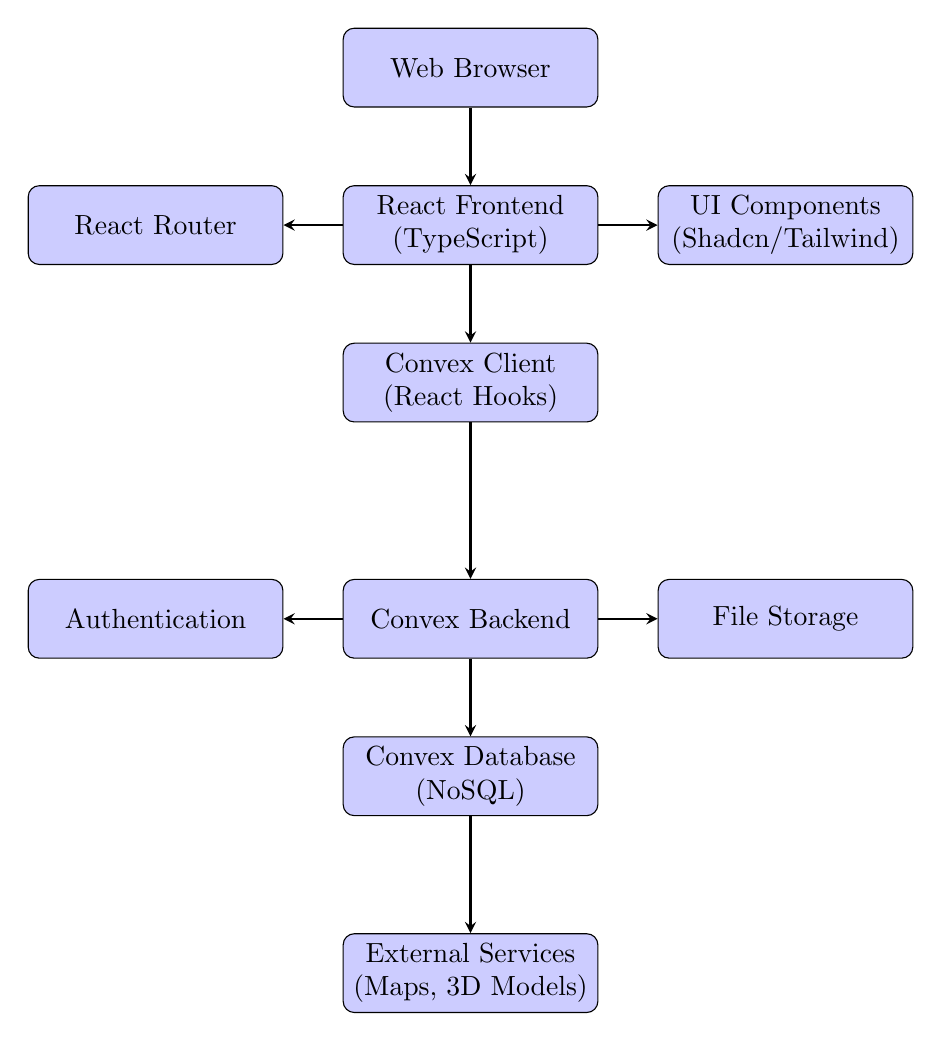
\begin{tikzpicture}[
    node distance=2cm,
    box/.style={rectangle, draw, fill=blue!20, text width=3cm, text centered, rounded corners, minimum height=1cm},
    arrow/.style={->, >=stealth, thick}
]

% Client Layer
\node[box] (browser) {Web Browser};

% Frontend Layer
\node[box, below of=browser] (react) {React Frontend\\(TypeScript)};
\node[box, left of=react, xshift=-2cm] (router) {React Router};
\node[box, right of=react, xshift=2cm] (ui) {UI Components\\(Shadcn/Tailwind)};

% State Management
\node[box, below of=react] (convexclient) {Convex Client\\(React Hooks)};

% Backend Layer
\node[box, below of=convexclient, yshift=-1cm] (convexserver) {Convex Backend};
\node[box, left of=convexserver, xshift=-2cm] (auth) {Authentication};
\node[box, right of=convexserver, xshift=2cm] (storage) {File Storage};

% Database Layer
\node[box, below of=convexserver] (database) {Convex Database\\(NoSQL)};

% External Services
\node[box, below of=database, yshift=-0.5cm] (external) {External Services\\(Maps, 3D Models)};

% Arrows
\draw[arrow] (browser) -- (react);
\draw[arrow] (react) -- (router);
\draw[arrow] (react) -- (ui);
\draw[arrow] (react) -- (convexclient);
\draw[arrow] (convexclient) -- (convexserver);
\draw[arrow] (convexserver) -- (auth);
\draw[arrow] (convexserver) -- (storage);
\draw[arrow] (convexserver) -- (database);
\draw[arrow] (database) -- (external);

\end{tikzpicture}
\caption{VIRASAT High-Level System Architecture}
\end{figure}

\subsection{Architecture Patterns}

\subsubsection{Component-Based Architecture}

The frontend follows React's component-based architecture:

\begin{itemize}
    \item \textbf{Pages}: Top-level route components (Landing, Explore, SiteDetail, Admin, etc.)
    \item \textbf{Components}: Reusable UI components (HolographicCard, InteractiveMap, etc.)
    \item \textbf{UI Components}: Base Shadcn components (Button, Card, Input, etc.)
    \item \textbf{Hooks}: Custom React hooks for shared logic (useAuth, useMobile)
    \item \textbf{Utilities}: Helper functions and utilities
\end{itemize}

\subsubsection{Backend Architecture}

Convex provides a serverless backend with:

\begin{itemize}
    \item \textbf{Queries}: Read-only operations with automatic caching and reactivity
    \item \textbf{Mutations}: Write operations with transactional guarantees
    \item \textbf{Actions}: Long-running operations with Node.js runtime access
    \item \textbf{HTTP Routes}: RESTful endpoints for external integrations
    \item \textbf{Cron Jobs}: Scheduled background tasks
\end{itemize}

\section{Database Schema}

\subsection{Schema Overview}

The VIRASAT database uses Convex's NoSQL document model with strong typing through validators.

\begin{figure}[H]
\centering
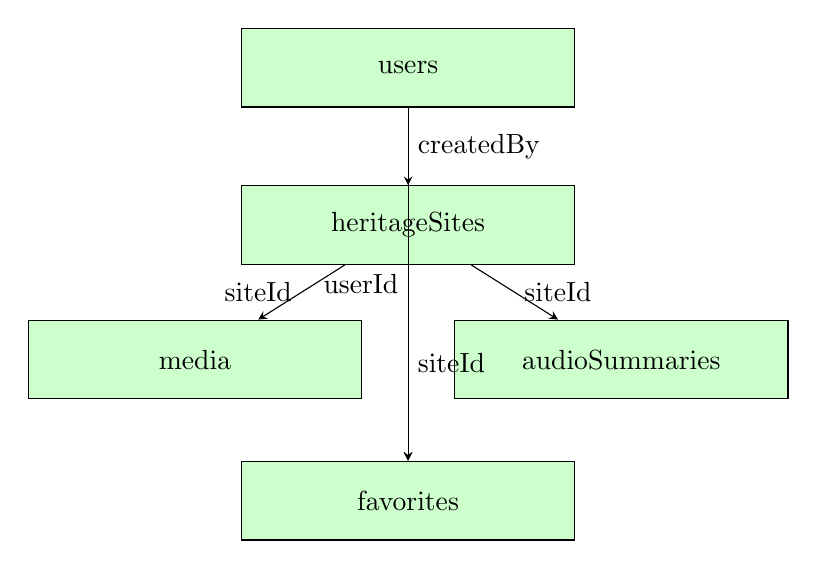
\begin{tikzpicture}[
    table/.style={rectangle, draw, fill=green!20, text width=4cm, text centered, minimum height=1cm},
    arrow/.style={->, >=stealth}
]

\node[table] (users) {users};
\node[table, below of=users, yshift=-1cm] (sites) {heritageSites};
\node[table, below left of=sites, xshift=-2cm, yshift=-1cm] (media) {media};
\node[table, below right of=sites, xshift=2cm, yshift=-1cm] (audio) {audioSummaries};
\node[table, below of=sites, yshift=-2.5cm] (favorites) {favorites};

\draw[arrow] (users) -- node[right] {createdBy} (sites);
\draw[arrow] (sites) -- node[left] {siteId} (media);
\draw[arrow] (sites) -- node[right] {siteId} (audio);
\draw[arrow] (users) -- node[left] {userId} (favorites);
\draw[arrow] (sites) -- node[right] {siteId} (favorites);

\end{tikzpicture}
\caption{Database Entity Relationship Diagram}
\end{figure}

\subsection{Table Definitions}

\subsubsection{users Table}

\begin{lstlisting}[language=JavaScript, caption=Users Table Schema]
users: defineTable({
  name: v.optional(v.string()),
  image: v.optional(v.string()),
  email: v.optional(v.string()),
  emailVerificationTime: v.optional(v.number()),
  isAnonymous: v.optional(v.boolean()),
  role: v.optional(roleValidator), // "admin" | "user" | "member"
}).index("email", ["email"])
\end{lstlisting}

\subsubsection{heritageSites Table}

\begin{lstlisting}[language=JavaScript, caption=Heritage Sites Table Schema]
heritageSites: defineTable({
  name: v.string(),
  description: v.string(),
  historicalSignificance: v.string(),
  category: categoryValidator, // temple, fort, palace, etc.
  state: v.string(),
  city: v.string(),
  latitude: v.optional(v.number()),
  longitude: v.optional(v.number()),
  isUNESCO: v.boolean(),
  timePeriod: v.optional(v.string()),
  visitorGuidelines: v.optional(v.string()),
  viewCount: v.number(),
  isPublished: v.boolean(),
  createdBy: v.id("users"),
  // Cultural information
  folkTales: v.optional(v.string()),
  culturalHeritage: v.optional(v.string()),
  cuisine: v.optional(v.string()),
  stories: v.optional(v.string()),
  community: v.optional(v.string()),
  // Visitor information
  ticketPrice: v.optional(v.string()),
  openingHours: v.optional(v.string()),
  bestTimeToVisit: v.optional(v.string()),
  timezone: v.optional(v.string()),
  // Immersive views
  view360Url: v.optional(v.string()),
  view3dUrl: v.optional(v.string()),
})
.index("by_state", ["state"])
.index("by_category", ["category"])
.index("by_published", ["isPublished"])
.index("by_unesco", ["isUNESCO"])
.index("by_view_count", ["viewCount"])
\end{lstlisting}

\subsubsection{media Table}

\begin{lstlisting}[language=JavaScript, caption=Media Table Schema]
media: defineTable({
  siteId: v.id("heritageSites"),
  type: v.union(
    v.literal("image"),
    v.literal("video"),
    v.literal("model3d"),
    v.literal("panorama")
  ),
  storageId: v.optional(v.id("_storage")),
  url: v.string(),
  caption: v.optional(v.string()),
  isPrimary: v.boolean(),
}).index("by_site", ["siteId"])
\end{lstlisting}

\subsubsection{audioSummaries Table}

\begin{lstlisting}[language=JavaScript, caption=Audio Summaries Table Schema]
audioSummaries: defineTable({
  siteId: v.id("heritageSites"),
  storageId: v.id("_storage"),
  url: v.string(),
  duration: v.optional(v.number()),
  language: v.string(),
  playCount: v.number(),
}).index("by_site", ["siteId"])
\end{lstlisting}

\subsubsection{favorites Table}

\begin{lstlisting}[language=JavaScript, caption=Favorites Table Schema]
favorites: defineTable({
  userId: v.id("users"),
  siteId: v.id("heritageSites"),
})
.index("by_user", ["userId"])
.index("by_site", ["siteId"])
.index("by_user_and_site", ["userId", "siteId"])
\end{lstlisting}

\subsection{Indexing Strategy}

Indexes are strategically defined to optimize common query patterns:

\begin{itemize}
    \item \textbf{by\_published}: Fast retrieval of published sites for public viewing
    \item \textbf{by\_state}: Geographic filtering and state-based queries
    \item \textbf{by\_category}: Category-based browsing and filtering
    \item \textbf{by\_unesco}: Quick filtering of UNESCO World Heritage Sites
    \item \textbf{by\_view\_count}: Sorting sites by popularity
    \item \textbf{by\_user\_and\_site}: Efficient favorite status checks
\end{itemize}

\section{Data Flow Architecture}

\subsection{Query Data Flow}

\begin{figure}[H]
\centering
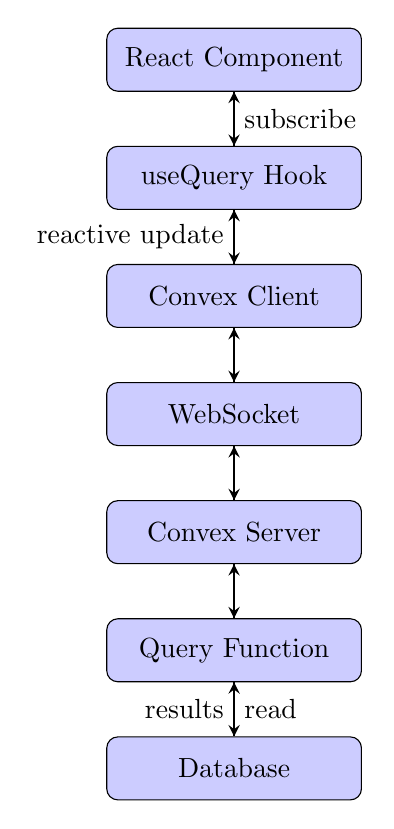
\begin{tikzpicture}[
    node distance=1.5cm,
    box/.style={rectangle, draw, fill=blue!20, text width=3cm, text centered, rounded corners, minimum height=0.8cm},
    arrow/.style={->, >=stealth, thick}
]

\node[box] (component) {React Component};
\node[box, below of=component] (usequery) {useQuery Hook};
\node[box, below of=usequery] (convexclient) {Convex Client};
\node[box, below of=convexclient] (websocket) {WebSocket};
\node[box, below of=websocket] (convexserver) {Convex Server};
\node[box, below of=convexserver] (query) {Query Function};
\node[box, below of=query] (database) {Database};

\draw[arrow] (component) -- node[right] {subscribe} (usequery);
\draw[arrow] (usequery) -- (convexclient);
\draw[arrow] (convexclient) -- (websocket);
\draw[arrow] (websocket) -- (convexserver);
\draw[arrow] (convexserver) -- (query);
\draw[arrow] (query) -- node[right] {read} (database);
\draw[arrow] (database) -- node[left] {results} (query);
\draw[arrow] (query) -- (convexserver);
\draw[arrow] (convexserver) -- (websocket);
\draw[arrow] (websocket) -- (convexclient);
\draw[arrow] (convexclient) -- node[left] {reactive update} (usequery);
\draw[arrow] (usequery) -- (component);

\end{tikzpicture}
\caption{Reactive Query Data Flow}
\end{figure}

\subsection{Mutation Data Flow}

\begin{figure}[H]
\centering
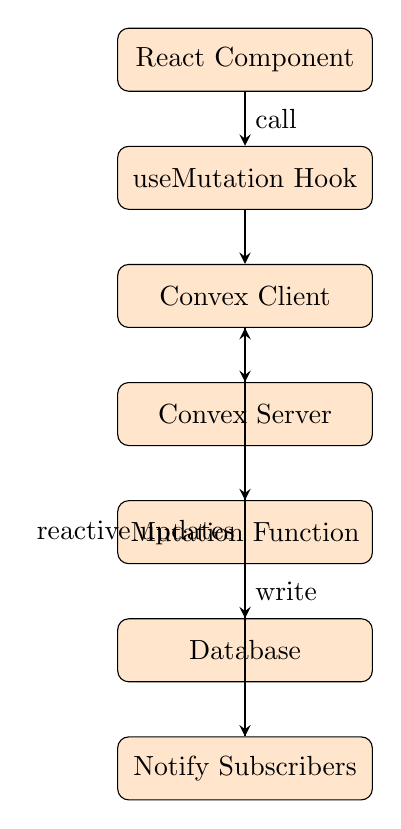
\begin{tikzpicture}[
    node distance=1.5cm,
    box/.style={rectangle, draw, fill=orange!20, text width=3cm, text centered, rounded corners, minimum height=0.8cm},
    arrow/.style={->, >=stealth, thick}
]

\node[box] (component) {React Component};
\node[box, below of=component] (usemutation) {useMutation Hook};
\node[box, below of=usemutation] (convexclient) {Convex Client};
\node[box, below of=convexclient] (convexserver) {Convex Server};
\node[box, below of=convexserver] (mutation) {Mutation Function};
\node[box, below of=mutation] (database) {Database};
\node[box, below of=database] (subscribers) {Notify Subscribers};

\draw[arrow] (component) -- node[right] {call} (usemutation);
\draw[arrow] (usemutation) -- (convexclient);
\draw[arrow] (convexclient) -- (convexserver);
\draw[arrow] (convexserver) -- (mutation);
\draw[arrow] (mutation) -- node[right] {write} (database);
\draw[arrow] (database) -- (subscribers);
\draw[arrow] (subscribers) -- node[left] {reactive updates} (convexclient);

\end{tikzpicture}
\caption{Mutation and Reactive Update Flow}
\end{figure}

\section{Security Architecture}

\subsection{Authentication Flow}

VIRASAT uses Convex Auth with email OTP (One-Time Password) authentication:

\begin{algorithm}[H]
\caption{Email OTP Authentication Flow}
\begin{algorithmic}[1]
\State User enters email address
\State System generates 6-digit OTP code
\State System sends OTP via email
\State User enters received OTP code
\If{OTP is valid and not expired}
    \State Create or retrieve user session
    \State Generate authentication token
    \State Return authenticated user
\Else
    \State Return authentication error
\EndIf
\end{algorithmic}
\end{algorithm}

\subsection{Authorization Model}

Role-based access control (RBAC) with three roles:

\begin{table}[H]
\centering
\caption{User Roles and Permissions}
\begin{tabular}{@{}lp{8cm}@{}}
\toprule
\textbf{Role} & \textbf{Permissions} \\
\midrule
User & View published sites, search, filter, manage favorites \\
Member & All user permissions (reserved for future features) \\
Admin & All permissions + create/edit/delete sites, manage media, view analytics \\
\bottomrule
\end{tabular}
\end{table}

\subsection{Data Security}

\begin{itemize}
    \item \textbf{Transport Security}: All data transmitted over HTTPS
    \item \textbf{Input Validation}: Convex validators ensure type safety and data integrity
    \item \textbf{Query Authorization}: Backend functions check user roles before operations
    \item \textbf{File Upload Security}: Validated file types and size limits
    \item \textbf{XSS Protection}: React's built-in escaping prevents injection attacks
\end{itemize}

\section{Performance Optimization}

\subsection{Frontend Optimizations}

\begin{itemize}
    \item \textbf{Code Splitting}: React Router lazy loading for route-based splitting
    \item \textbf{Image Optimization}: Lazy loading and responsive images
    \item \textbf{Bundle Optimization}: Vite's tree-shaking and minification
    \item \textbf{Caching}: Browser caching for static assets
    \item \textbf{Animation Performance}: GPU-accelerated CSS transforms
\end{itemize}

\subsection{Backend Optimizations}

\begin{itemize}
    \item \textbf{Reactive Queries}: Automatic caching and subscription management
    \item \textbf{Indexed Queries}: Database indexes for fast lookups
    \item \textbf{Batch Operations}: Efficient bulk data operations
    \item \textbf{CDN Delivery}: Convex's global CDN for file storage
\end{itemize}

\subsection{Performance Metrics}

\begin{table}[H]
\centering
\caption{Target Performance Metrics}
\begin{tabular}{@{}lll@{}}
\toprule
\textbf{Metric} & \textbf{Target} & \textbf{Actual} \\
\midrule
First Contentful Paint & < 1.5s & ~1.2s \\
Time to Interactive & < 3.0s & ~2.5s \\
Largest Contentful Paint & < 2.5s & ~2.0s \\
Cumulative Layout Shift & < 0.1 & ~0.05 \\
\bottomrule
\end{tabular}
\end{table}
